%%%%%%%%%%%%%%%%%%%%%%% file typeinst.tex %%%%%%%%%%%%%%%%%%%%%%%%%
%
% This is the LaTeX source for the instructions to authors using
% the LaTeX document class 'llncs.cls' for contributions to
% the Lecture Notes in Computer Sciences series.
% http://www.springer.com/lncs       Springer Heidelberg 2006/05/04
%
% It may be used as a template for your own input - copy it
% to a new file with a new name and use it as the basis
% for your article.
%
% NB: the document class 'llncs' has its own and detailed documentation, see
% ftp://ftp.springer.de/data/pubftp/pub/tex/latex/llncs/latex2e/llncsdoc.pdf
%
%%%%%%%%%%%%%%%%%%%%%%%%%%%%%%%%%%%%%%%%%%%%%%%%%%%%%%%%%%%%%%%%%%%


\documentclass[runningheads,a4paper]{llncs}

\usepackage{amssymb}
\setcounter{tocdepth}{3}
\usepackage{graphicx}
\usepackage{url}
\usepackage{fancyvrb}
\usepackage{hyperref}
\usepackage{amsmath,latexsym}
\usepackage[utf8x]{inputenc}
\usepackage[spanish]{babel}
\urldef{\mailsa}\path|astradalucasezequiel@gmail.com|
\urldef{\mailsb}\path|marianvanetta@hotmail.com
|    


\begin{document}

\mainmatter  % start of an individual contribution

% first the title is needed
\title{EasyCrypt: análisis de la herramienta.}

% a short form should be given in case it is too long for the running head
%%\titlerunning{Analisis de Herramienta, EasyCrypt}

% the name(s) of the author(s) follow(s) next
%
% NB: Chinese authors should write their first names(s) in front of
% their surnames. This ensures that the names appear correctly in
% the running heads and the author index.
%
\author
{
Astrada Lucas Ezequiel
y
Vanetta Mariano
}
%
%%\authorrunning{Analisis de Herramienta, EasyCrypt}
% (feature abused for this document to repeat the title also on left hand pages) Aca sirve par el encabezado de pagina

% the affiliations are given next; don't give your e-mail address
% unless you accept that it will be published
\institute{Universidad Nacional de Córdoba\\
Facultad de Matemática, Física, Astronomía y Computación\\
\mailsa\\
\mailsb\\
\url{https://www.famaf.unc.edu.ar/}}

%
% NB: a more complex sample for affiliations and the mapping to the
% corresponding authors can be found in the file "llncs.dem"
% (search for the string "\mainmatter" where a contribution starts).
% "llncs.dem" accompanies the document class "llncs.cls".
%

%%\toctitle{Analisis de Herramienta, EasyCrypt}
\toctitle{EasyCrypt}
\maketitle


\begin{abstract}    
EasyCrypt es un conjunto de herramientas para razonar sobre las propiedades reales de los cálculos probabilísticos con código contradictorio. Su aplicación principal es la construcción y verificación de pruebas criptográficas basadas en juegos. 
Es un marco formado por un lenguaje de programación junto a un motor de resolución de lógica de Hoare Relacional Probabilística. A lo largo de este documento se discutirá sobre dicha herramienta, desde su historia hasta casos prácticos que la utilizan.
\cite{article1}


\keywords{EasyCrypt  \and Pruebas criptográficas \and Juegos  \and Probabilístico.}
\end{abstract}


\section{Introducción}
La criptografía desempeña un papel clave en la seguridad de la comunicación moderna e infractucturas informáticas.  Por este motivo es de suma importancia diseñar sistemas criptográficos que proporcionen grandes garantías de seguridad.
La sociedad depende hoy más que nunca de la tecnología, pero la inversión en seguridad es escasa y los riesgos de usar sistemas informáticos son cada día mayores. La criptografía es una de las piedras angulares de la seguridad en este  ámbito, por lo que recientemente se ha dedicado una cantidad considerable de recursos al desarrollo de herramientas que ayuden en la evaluación y mejora de los algoritmos criptográficos. EasyCrypt es uno de estos sistemas.

EasyCrypt busca simplificar pruebas de seguridad de altísima complejidad y mejorar los tiempos de respuestas de las mismas. En la sección 2 y 3 se introduce el contexto de creación del programa. La sección 4 analizará la usabilidad que brinda EasyCrypt al usuario. Las especificaciones técnicas, comparaciones con otros programas y casos de uso se encontrarán en las secciones 5, 6 y 7 respectivamente. Por último, en la sección 8 enunciaremos nuestra conclusión y opiniones sobre EasyCrypt.
    
\section{Contexto de creación de la herramienta}
El desarrollo de EasyCrypt se inició en 2009 y el prototipo inicial se usó para probar la seguridad de varias construcciones, incluso el esquema de cifrado Cramer-Shoup, el diseño de la función de hash iterativa Merfle-Damgaard y el esquema de cifrado ZEAP. EasyCrypt ha sido desarrollado inicialmente por el Instituto de Software \href{http://www.imdea.org/es}{IMDEA} (Institutos Madrileños de Estudios Avanzados) e \href{https://www.inria.fr/en/}{Inria} (Instituto de Investigacion para Ciencias Digitales). Actualmente se desarrolla en el Instituto IMDEA Software, Inria y \href{https://www.polytechnique.edu/}{École Polytechnique} (Instituto Público Francés de Educación Avanzada e Investigación). EasyCrypt es un proyecto de software libre, distribuido bajo los términos de la licencia CeCILL-B, y su código fuente está accesible desde la página del proyecto. 
La versión actual de EasyCrypt (versión 1.0), lanzada el 10 Octubre 2017, aún está en desarrollo. 
\cite{article2}

\section{Objetivo de la herramienta} 
Uno de los componentes básicos de prácticamente cualquier sistema de seguridad es la criptografía. Su utilidad no se limita a impedir que una persona no autorizada con acceso a datos privados pueda entenderlos (cifrado), si no que también cubre otras necesidades como la verificación de la identidad (autenticación) o la de poder garantizar de que una información no ha sido alterada (integridad). Por lo general estas primitivas criptográficas basan su seguridad en la dificultad computacional que tiene resolver ciertos problemas. Para estar seguros de que los mecanismos criptográficos realmente cumplen con su cometido, es necesario someterlos a un proceso de verificación riguroso. El objetivo es poder razonar sobre ellos y demostrar que cumplen ciertas propiedades de seguridad. 

Esta herramienta apunta a solucionar problemas de seguridad. EasyCrypt usa varios lenguajes de programación distintos a la hora de evaluar un código fuente. Esta es una herramienta que se utiliza en las etapas de desarrollo y testing de software. Funciona como un intérprete de un lenguaje de propósito general y de forma interactiva: cuando se le proporciona un archivo a evaluar, lo recorre de arriba hacia abajo comprobando que todos los pasos de las demostraciones son correctos. Usando Proof General, un modo de editor de texto EMACS, es posible editar un archivo mientras el intérprete lo va emulando sobre la marcha, ayudando y guiando al usuario a medida que éste desarrolla cada demostración. 

\section{Descripción de la herramienta del lado del usuario}

EasyCrypt tiene su propio programa para ser utilizado el cual puede ser descargado desde GitHub.\cite{link1}
EasyCrypt también se utiliza en la terminal de comando y tiene un funcionamiento muy simple pero poco intuitivo. Se ingresa el código a evaluar y al ejecutarlo este lo analiza línea por línea hasta llegar a un resultado o error. Por eso, es más conveniente utilizar EMACS\cite{link2}. EMACS es un editor de texto que tiene un inteprete de Turing Completo, el cual usa el lenguaje ELisp. Puede ser instalado en los 3 sistemas operativos más utilizados: Windows, Mac OS y distribuciones de Linux. Utiliza archivos *.ec. Es un programa en el cual la visualización de los elementos es más amigable con el usuario. Tiene por un lado el archivo selecionado y por otro las ejecuciones realizadas. La interfaz permite analizar el archivo paso por paso (next) o ejectutarlo completamente (use), volver pasos atrás (undo), revisar cual es el estado en determinada línea (state), entre otras opciones.


\section{Aspectos técnicos}
EasyCrypt trabaja con enfoque basado en juegos, cuyos principales actores son los ADVERSARIOS, los cuales son procesos Abstractos y los ORÁCULOS, que son procesos definidos. La herramienta contiene variables globales y una colección de los procesos ya mencionados.

Éste posee 4 caracteristicas principales:
\begin{itemize}
	\item \textbf{Lenguaje de programacion}:
El lenguaje utilizado es pWhile el cual es de tipado fuerte, imperativo probabilistico:

\begin{Verbatim}
	C ::= skip		 nop
	|V <- E		    deterministic assignment
	|V <- DE		   probabilistic assignment
	|if E then C else C	conditional
	|while E do C	      loop
	|V <- P(E, . . . , E)      procedure call
	|C; C		      sequence
Donde V = {variables identificadora}, P = {nombres de procesos},
 E = {expresiones de prueba}, DE ={set de expresiones probabilisticas}
\end{Verbatim}

	\item \textbf{Semántica Denotacional}:
Estos programas son interpretados como funciones, que se mapean en la memoria.

	\item \textbf{Logica Relacional}: Se utiliza el método probabilístico RELATIONAL HOARE LOGIC (pRHL):
		
\centerline{$\models$ c1 $\sim$ c2 : $\Psi$ $\implies$ $\Phi$}	
			
donde c1,c2 son programas probabilísticos y los símbolos corresponden a la pre y post condición.

Dentro de EasyCrypt la gramática es la siguiente:

\centerline{$\Psi$, $\Phi$ ::= e $\mid$ $\neg$ $\Phi$ $\mid$ $\Psi$ ∧ $\Phi$ $\mid$ $\Psi$ ∨ $\Phi$ $\mid$ $\Psi$ $\implies$ $\Phi$ $\mid$ $\forall$ x. $\Phi$ $\mid$ $\exists$ x. $\Phi$}

donde la e corresponde a una expresión booleana.


	\item \textbf{Razonamiento probabilístico}:
Estos razonamientos se expresan en términos de eventos probabilísticos y no como juicios de pRHL.\cite{article3}

\end{itemize}
En caso de que EasyCrypt encuentre un evento fallido, su razonamiento se va a basar en el siguiente lema:
\begin{lemma}{Lema Fundamental:}
Sea $G_1$ , $G_2$ dos juegos y A, B y F tres eventos tales que

\[|= G_1 ∼ G_2 : \Psi \implies (F(1) \leftrightarrow F(2)) \land (\neg F(1) \rightarrow (A(1) \leftrightarrow B(2)))\]
Luego, si $m_1$ $\Psi$ $m_2$ ,
\begin{enumerate}
	\item Pr [$G_1$ , $m_1$ : A $\land$ $\neg$F ] = Pr [$G_2$ , $m_2$ : B $\land$ $\neg$ F ],
	\item Pr [$G_1$ , $m_1$ : A] − Pr [$G_2$ , $m_2$ : B] $\leq$  Pr [$G_1$ , $m_1$ : F ] = Pr [$G_2$ , $m_2$ : F ]
\end{enumerate}
\end{lemma}

Este Lema permite unir las diferencias entre la probabilidad de un evento A en el juego $G_1$ y la posible diferencia del evento B en el juego $G_2$ por la probabilidad de F en cualquier juego.\cite{article4}


Otra caracteristica de EasyCrypt es su manera de reducir abstractos mediante la utilizacion del calculo lambda, particularmente estos tres metodos:

\begin{itemize}

	\item \textbf{Call-by-name}: reduce la expresión de más afuera de la izquierda salvo que este en forma normal débil. No es estricta.

	\item \textbf{Call-by-value}: reduce la expresión de más adentro de la izquierda, salvo que este en forma normal débil. Es estricta.

	\item \textbf{Applicative order}: reduce la expresión de más adentro a la izquierda, salvo que este de forma normal. Es estricta.
\end{itemize}

Las respuestas que brinda EasyCrypt son esquemas de pruebas que incrementan la confianza en las respuestas produciendo pruebas verificables independientes \ref{fig1}. También permite generar pruebas en formato COQ (las cuales son generadas en otro archivo), para que luego el usuario si lo desea, las ejecute en dicho formato con dicho programa.\cite{article4}

\begin{figure}
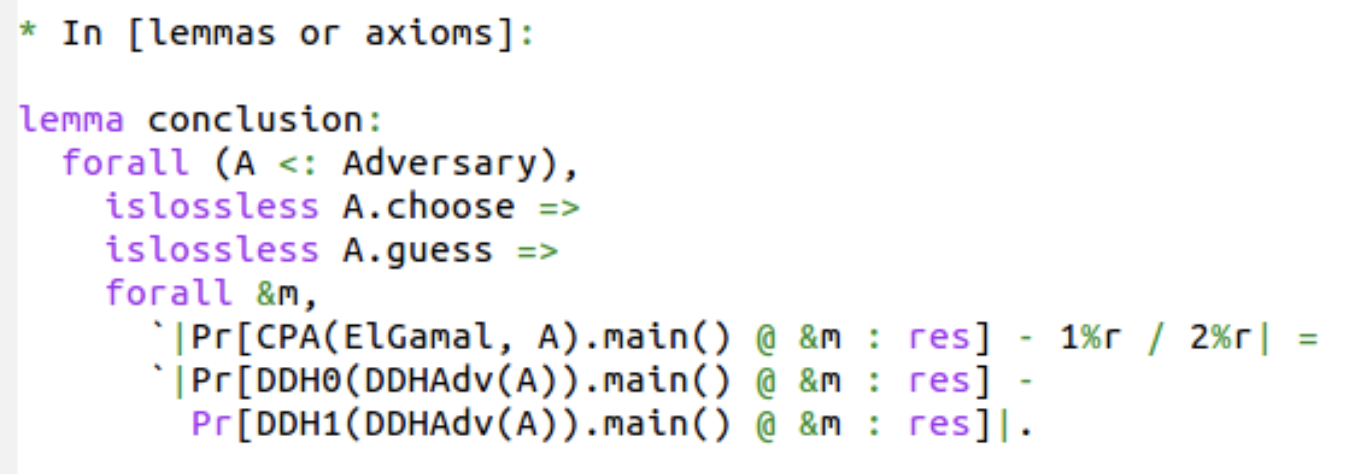
\includegraphics[width=\textwidth, height=3.5cm]{fig1.png}
\caption{En dicha figura se puede observar el resultado de una ejecución exitosa de ElGamal, el cual fue uno de los primeros problemas criptograficos importantes, utilizando EasyCrypt.} \label{fig1}
\end{figure}


\section{Comparación de programas}
\centerline{\textbf{{\emph{CertiCrypt}}}}
En la parte programacional, EasyCrypt no posee procesos recursivos, CertiCrypt\cite{link3} si. En el caso de las evidencias generadas, EasyCrypt es parcial por no tener generadores de pruebas COQ (se está buscando agregar esta característica). Este también genera pruebas en base a la probabilidad y no máquinas totalmente probadas. Se podria considerar que EasyCrypt tiene como antecesor a CertiCrypt siendo EasyCrypt ampliamente eficaz a la hora de resolver problemas criptograficos.

\begin{table}
  \caption{Comparación de EasyCrypt con CertiCrypt}
  \label{tab:simple1}
  \centering
  \begin{tabular}{ |p{3.5cm}|p{1cm}|p{1.5cm}|p{1cm}|p{1.5cm}|p{1cm}|p{1.5cm}|  }
 \hline
 & \multicolumn{2}{|c|}{CertiCrypt} & \multicolumn{2}{|c|}{EasyCrypt} & \multicolumn{2}{|c|}{Extracted} \\\cline{2-7}

 &Lines&Time&Lines&Time&Lines&Time\\\cline{2-7}
 \hline
 ElGamal(IND-CPA) & 565 & 45s & 190 & 12s & 1130 & 23s\\
 Hashed ElGamal(IND-CPA) & 1255  & 1m 5s & 243  & 33s & 1772 & 41s\\
 Full-Domain Hash(EF-CMA) & 2035 & 5m 46s&  509 & 1m 26s & 2724 & 1m11s\\
 Cramer-Shoup(IND-CCA) & n/a & n/a & 1637 & 5m 12s & 5504 & 3m14s\\
 \hline
\end{tabular}
\end{table}

Hardware para esta prueba: procesador 2.8GHz Intel Core 2 Duo con 4GB de RAM en Mac OS X 10.6.7.\cite{article3}

Con el gráfico \ref{tab:simple1} anterior podemos concluir que la mayor diferencia entre estos dos programas es la rapidez y facilidad en la construcción de pruebas.

\centerline{\textbf{{\emph{CRYPTHOL}}}}

En la semántica, EasyCrypt soporta distribuciones de probabildad discretas, todas expresadas usando el lenguaje pWhile. CryptHOL\cite{link4} tiene el mismo dominio y el lenguaje es igual de expresivo gracias al operador de punto fijo. A diferencia del lenguaje imperativo usado por EasyCrypt, CryptHOL utiliza lenguaje funcional embebido.

CryptHOL crea su dominio semántico atraves de los principios de HOL y tiene un asistente de prueba (COQ o Isabelle) para corroborar las derivaciones de las reglas de prueba. En cambio EasyCrypt no posee ningún asistente para las pruebas, entonces hay que confiar en que las implementaciones en OCaml y en que los solucionadores externos SMT sean correctas.

Otra diferencia importante radica en las librerías disponibles. Como ya mencionamos, EasyCrypt no posee asistentes de pruebas, por lo tanto tiene librerías muy chicas que le permite razonar sobre programas rápidamente, a diferencia de CryptHOL, que al estar enfocado en resolver matemática pura, necesita de librerías completas que son brindadas por Isabelle/HOL o COQ.

En ambos programas la eficiencia de cómputos no puede ser expresada formalmente porque sus logicas identifican términos hasta ciertos computos, por ejemplo, ($\lambda$x. x+x) no puede ser distinguido del valor 2.\cite{article6}

\begin{table}
  \caption{Comparación de EasyCrypt con CryptHOL}
  \label{tab:simple2}
  \centering
  \begin{tabular}{ |p{4cm}|p{3.5cm}|p{2cm}|p{2cm}|  }
 \hline
 Algoritmo Criptográfico & Propiedad de Seguridad & CryptHOL & EasyCrypt\\\cline{1-4}
 \hline
 RP-RF switching lemma &  & 120ms & 448ms\\
 Elgamal & IND-CPA & 49ms  & 68ms\\
 Hashed Elgamal in the ROM & IND-CPA & 253ms &  216ms\\
 \hline
\end{tabular}
\end{table}


El cuadro\ref{tab:simple2} anterior es una comparacion entre EasyCrypt y CryptHOL probando tres algoritmos criptograficos.No se encontró el hardware utilizado para la comparacion de Cuadro2\ref{tab:simple2}.




\section{Casos de estudio}
EasyCrypt es una herramienta muy potente para probar problemas de seguridad, por lo tanto los siguientes casos de estudio hacen referencia en mayor medida a la criptografía.


\centerline{\textbf{{\emph{Hashed ElGamal}}}}


Hashed ElGamal es una variante de encriptación ElGamal con seguridad IND-CPA, la cual puede ser reducida a lo siguiente (Computational Diffie-Hellman): es difícil computar $g^{x*y}$ dado $g^x$ y $g^y$ donde x e y son eventos aleatorios uniformes dentro de $\mathbb{Z}_q$.
Para esta prueba primero es necesario expresar los cinco ingredientes para el input de EasyCrypt:
\begin{itemize}
	\item Tipo, constantes y declaraciones del operador.
	\item Axiomas.
	\item Definiciones del Juego.
	\item Juicios en pRHL.
	\item Afirmaciones de probabildad.
\end{itemize}

El resultado de la prueba fue que la reducción de código es sustancial tanto que es 5 veces más chica que la inicial asi también como el desempeño de EasyCrypt (medido en tiempo) fue de 33 segundos.\cite{article3}




\centerline{\textbf{{\emph{Cramer-Shoup Cryptosystem}}}}

Cramer-Shoup Cryptosystem es una encripción de llave pública basada en la encriptación ElGramal. Este caso se hizo famoso ya que fue el primer encriptador asimétrico eficiente. La idea es probar que es seguro contra ataques de texto cifrado elegido adaptativos (o en inglés Adaptive Chosen-Ciphertext).
Mediante las siguientes pruebas se puede probar el teorema de Cramer-Shoup:
\emph{Las siguientes definiciones y teoremas fueron citados en su idioma de origen, con la finalidad de no perder su verdadero significado.}
\begin{definition}{Target Collision-Resistance}

Sea $H_k : A \rightarrow B_{k∈K}$ be a keyed family of hash
functions. The advantage of an adversary $\mathcal{C}$ against the target collision-resistance of H is defined as

	\[Adv_{TCR}^\mathcal{C} = Pr[TCR:H_k(x) = H_k (y) \land x \neq y]\]
	donde el experimento TCR se define mediante el siguiente juego:
	\[Game TCR : x \leftarrow C 1 ( ); k \leftarrow K; y \leftarrow \mathcal{C}(k)\]
\end{definition}

\begin{definition}{CCA-advantage}
Let ($\mathcal{K}\mathcal{G}$, $\mathcal{E}$, $\mathcal{D}$) un asymmetric encryption scheme. The CCA-advantage of an adversary $\mathcal{A}$ limited to $q_\mathcal{D}$ decryption queries against the adaptive chosen-ciphertext security of the scheme is defined as

\[Adv_{CCA}^\mathcal{A} (q_\mathcal{D})= |Pr[IND-CCA: b=b'] - \frac{1}{2}\]
\end{definition}

\begin{theorem}{Cramer-Shoup Security}
Let $\mathcal{A}$ be an adversary against the IND-CCA security
of Cramer-Shoup limited to $q_\mathcal{D}$ decryption queries. Then, there exists an algorithm $\mathcal{B}$ for solving the
DDH problem in $\mathcal{G}$ and an adversary $\mathcal{C}$ against the target collision-resistance of the hash function H
such that
\[Adv_{CCA}^\mathcal{A}(q_\mathcal{D}) \leq Adv_{DDH}^\mathcal{B} + Adv_{TCR}^\mathcal{C} + \frac{q_\mathcal{D}^4}{q^4} + \frac{q_\mathcal{D} + 2}{q}\]
\end{theorem}

La prueba fue exitosa para cualquier consulta de descifrado (decryption query) bajo la condicion de u =! u'\cite{article3}

\centerline{\textbf{{\emph{CMAC, Caso de estudio Elegido}}}}
CMAC fue propuesto por Iwata y Kurosawa con el nombre de OMAC1, el cual cuenta con una prueba criptográfica basada en juegos muy compleja. Luego se fue transformando hasta llegar al CBC-MAC (bloque cifrado en cadena-código de autentificación del mensaje, o su nombre en inglés: cipher block chaining-message authentication code). En este, el mensaje es dividido en lista de bloques. Cada bloque es enmascarado usando el resultado del cifrado de bloque anterior, con esta dependencia se asegura que si se cambia un bit  del mensaje, el resto cambiara inpredeciblemente.

Los MAC cuentan con tres algoritmos (generador de clave, tagueo y de verificación). Éstos deben cumplir con las siguientes características: deben ser correctos, seguros y determinísticos, a diferencia de los BCB que solo requieren ser seguros.

Para realizar la prueba de CMAC se necesita probar que:

\centerline{\emph{ECBC es una MAC segura}}
\centerline{$\land$}
\centerline{\emph{FCBC es perfectamente indistinguible de ECBC}}
\centerline{$\land$}
\centerline{\emph{XCBC es computacionalmente indistinguible FCBC}}
\centerline{$\land$}
\centerline{\emph{CMAC es computacionalmente indistinguible de FCBC}}

\begin{itemize}
	\item \textbf{Seguridad ECBC}: se define como una noción basada en juego, mediante el juego de colisión de nombre, en donde al adversario $\mathcal{A}$ se le provee una lista de mensajes a su elección, antes de que la función hash f sea seleccionada de H. Éste gana si contiene dos mensajes distintos con la misma imagen de h. Se dice que una función hash f es resistente a colisión si la probabilidad es baja. Formalizando, la resistencia a la colisión de CBC-MAC es una familia de funciones hash indexada por un bloque de clave de cifrado. Esto produce un límite concreto en la seguridad de ECBC.
	\item \textbf{Seguridad FCBC}: La seguridad FCBC es esquivalente a ECBC, esto es gracias a que la composición de dos permutaciones aleatorias independientes quedan independientes de una de las permutaciones 
	\item \textbf{Seguridad XCBC}: La prueba de XCBC es indistinguible de FCBC. Se basa en que un adversario con oráculo accede a dos permutaciones aleatorias independientes $x_1$ y $x_2$ no pueden ser distinguidas de los oráculos $\pi (\cdot)$ y $\pi (k \oplus \cdot)$ cuando $\pi$ es una permutación aleatoria y k es elegida uniforme al azar e independientemente de $\pi$.
	\item \textbf{Seguridad CMAC}: La idea de esta seguridad de prevenir que el adversario acceda directamente el bloquede de cifrado del oráculo anadiendo una variable aleatoria independiente.
\end{itemize}
El caso fue exitoso ya que probó que CMAC es computacionalmente es indistinguible de FCBC, así como también los lemas utilizado para la prueba. Asi tambien CMAC permitio agregarle mas estructura a EasyCrypt y ayudarla en su crecimiento.\cite{article5}

\section{Conclusión}


EasyCrypt es un programa que, para su objetivo, es muy eficiente ya que las verficaciones que brinda son mucho más sencillas. Las actualizaciones que esperan sumar a la herramienta, aumentarían la calidad y espectro de las respuestas que brinda, como por ejemplo agregarle asistentes como COQ. En comparación a los otros programas y con la gran necesidad de seguridad en estos dias, EasyCrypt es una excelente herramienta con mucho potencial.

A nivel de usuario, lo único positivo que tiene es que es sencillo instalarlo, porque la interfaz gráfica propia de EasyCrypt presenta dificultades para su uso y no es intuitiva. Con respecto a EMACS, podemos mencionar que este tiene más facilidades pero aun así los archivos a analizar no son nada sencillos y la información no abunda en la parte práctica probablemente porque aún es una herramienta nueva y en constante cambio.



\begin{thebibliography}{1}
\bibitem{article1}
Gilles Barthe François Dupressoir,Benjamin Grégoire,César Kunz, Benedikt Schmidt and Pierre-Yves Strub : EasyCrypt: A Tutorial. 
\bibitem{article2}
EasyCrypt Reference Manual.
%\bibitem{article4}
%Guillermo Ramos Gutiérrez: Desarrollo de  funcionalidad para un% marco orientado sobre algoritmos criptográficos.%
\bibitem{article3}
Gilles Barthe, Benjamin Grégoire, Sylvain Heraud, Santiago Zanella Béguelin: Computer-Aided Security Proofs
for the Working Cryptographer.
\bibitem{article4}
Guillermo Ramos Gutiérrez: Implementing a term rewriting
engine for the EasyCrypt framework.
\bibitem{article5}
Cécile Baritel-Ruet, François Dupressoir, Pierre-Alain Fouque, Benjamin Grégoire. Formal Security.
Proof of CMAC and Its Variants. CSF 2018 - 31st EEE Computer Security Foundations Symposium,
Jul 2018, Oxford, United Kingdom.
\bibitem{article6}
David A. Basin, Andreas Lochbihler, and S. Reza Sefidgar: CryptHOL: Game-based Proofs in
Higher-order Logic.
\bibitem{link1}
Descarga e instalación EasyCrypt https://github.com/EasyCrypt/easycrypt
\bibitem{link2}
Descarga e instalacion EMACS https://www.easycrypt.info/binaries/ 
\bibitem{link3}
Pagina oficial CeriCrypt http://certicrypt.gforge.inria.fr/
\bibitem{link4}
Pagina oficial CryptHOL https://www.isa-afp.org/entries/CryptHOL.html
\end{thebibliography}
\end{document}
